\begin{figure}[tbp]
\centering
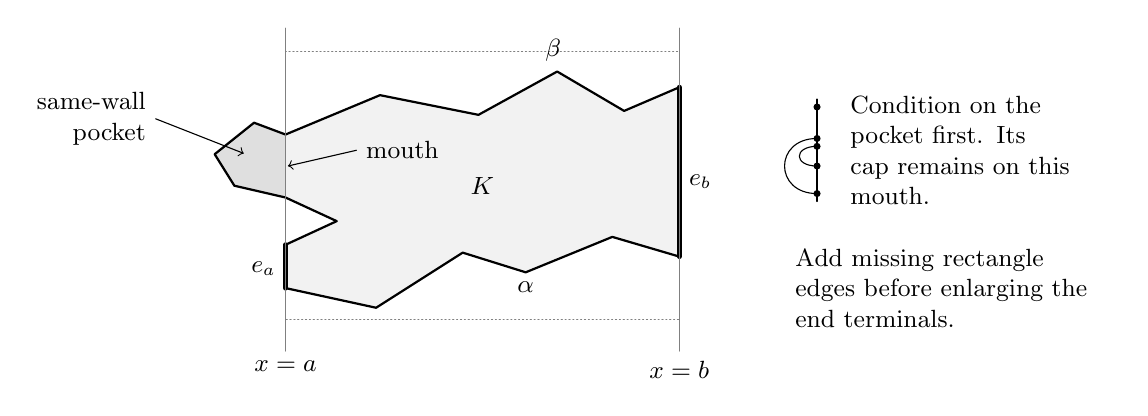
\begin{tikzpicture}[x=1cm,y=1cm,font=\small,line cap=round,line join=round]
  \draw[gray,densely dotted] (0,.25) rectangle (5,3.65);
  \path[fill=gray!10] (0,.65) -- (1.15,.4) -- (2.25,1.1) -- (3.05,.85) -- (4.15,1.3) -- (5,1.05)
    -- (5,3.2) -- (4.3,2.9) -- (3.45,3.4) -- (2.45,2.85) -- (1.2,3.1) -- (0,2.6)
    -- (0,1.8) -- (.65,1.5) -- (0,1.2) -- cycle;
  \path[fill=gray!25] (0,1.8) -- (-.65,1.95) -- (-.9,2.35) -- (-.4,2.75) -- (0,2.6) -- cycle;
  \draw[thick] (0,.65) -- (1.15,.4) -- (2.25,1.1) -- (3.05,.85) -- (4.15,1.3) -- (5,1.05);
  \draw[thick] (0,1.2) -- (.65,1.5) -- (0,1.8) -- (-.65,1.95) -- (-.9,2.35) -- (-.4,2.75)
    -- (0,2.6) -- (1.2,3.1) -- (2.45,2.85) -- (3.45,3.4) -- (4.3,2.9) -- (5,3.2);
  \draw[line width=1.8pt] (0,.65) -- (0,1.2);
  \draw[line width=1.8pt] (5,1.05) -- (5,3.2);
  \draw[densely dashed] (0,1.8) -- (0,2.6);
  \draw[gray] (0,-.15) -- (0,3.95);
  \draw[gray] (5,-.15) -- (5,3.95);
  \node[below] at (0,-.15) {$x=a$};
  \node[below] at (5,-.15) {$x=b$};
  \node[left] at (0,.9) {$e_a$};
  \node[right] at (5,2) {$e_b$};
  \node at (2.5,1.95) {$K$};
  \node[above] at (3.4,3.4) {$\beta$};
  \node[below] at (3.05,.85) {$\alpha$};
  \draw[<-] (-.53,2.36) -- (-1.65,2.8);
  \node[anchor=east,align=right] at (-1.65,2.8) {same-wall\\pocket};
  \draw[<-] (.03,2.2) -- (.9,2.4);
  \node[anchor=west] at (.9,2.4) {mouth};
  \draw (6.75,1.75) -- (6.75,3.05);
  \fill (6.75,1.85) circle (.045);
  \fill (6.75,2.2) circle (.045);
  \fill (6.75,2.45) circle (.045);
  \fill (6.75,2.55) circle (.045);
  \fill (6.75,2.95) circle (.045);
  \draw (6.75,1.85) .. controls (6.2,1.85) and (6.2,2.55) .. (6.75,2.55);
  \draw (6.75,2.2) .. controls (6.45,2.2) and (6.45,2.45) .. (6.75,2.45);
  \node[align=left,anchor=west,text width=3.2cm] at (7.05,2.4)
    {Condition on the pocket first. Its cap remains on this mouth.};
  \node[align=left,anchor=west,text width=4cm] at (6.35,.65)
    {Add missing rectangle edges before enlarging the end terminals.};
\end{tikzpicture}
\caption{A slab core cut from a winding corridor (schematic; lattice steps are suppressed). Consecutive opposite-wall cuts $e_a,e_b$ retain the ends. Same-wall excursions beyond a slab level are pockets, removed along their mouths to obtain $K$. Each pocket induces a separate noncrossing cap on its own mouth. The rectangle comparison preserves these caps while adding missing edges; only afterwards are the contact intervals merged with their respective terminals.}
\label{fig:slab-pockets}
\end{figure}
